\bookchapter{Bab 42: Panorama Model Besar dan Praktik API}

\chapterintro{Beberapa bab sebelumnya membahas “cara berkolaborasi dengan AI”; bab ini menjawab pertanyaan yang lebih mendasar: “AI mana yang dipakai? Bagaimana memakainya?” Lanskap model besar per Agustus 2026 sudah sangat kaya — di ranah internasional GPT, Claude, dan Gemini bersaing sebagai tiga raksasa; di Tiongkok DeepSeek, Tongyi Qianwen, GLM, Kimi, dan Doubao bermekaran. Setiap model punya karakter dan keahlian khasnya masing-masing: memilih yang tepat membuat pekerjaan jauh lebih efisien, memilih yang salah membuat pekerjaan terasa dua kali berat. Bab ini tidak hanya memperkenalkan model-model tersebut, tetapi juga mengajarkan cara menghubungkannya ke aplikasimu melalui API, serta cara memilih Token Plan (paket kuota) yang sesuai dengan kebutuhanmu.}

\booksection{Model Besar Internasional Utama: Format Tiga Raksasa}

Pasar model besar internasional per Agustus 2026 membentuk format tiga raksasa: OpenAI (seri GPT), Anthropic (seri Claude), dan Google (seri Gemini). Masing-masing punya karakter khas yang menonjol — mari kita kenali satu per satu.

\booksubsection{Seri OpenAI GPT-5.6: Jagoan Serba Bisa yang Seimbang}

OpenAI adalah pembuka gelombang model besar, dan seri GPT hingga kini tetap menjadi model yang paling banyak digunakan di dunia. Seri GPT-5.6 yang dirilis Juli 2026 memakai strategi tiga segmen: varian flagship GPT-5.6 Sol untuk kebutuhan reasoning kelas atas, varian seimbang GPT-5.6 Terra untuk pengembangan harian, dan varian ringan GPT-5.6 Luna untuk skenario konkurensi tinggi dengan biaya rendah. Ketiga model berbagi jendela konteks 1,05 juta Token, dan semuanya mendukung input gambar, function calling, serta output terstruktur.

\begin{center}
\begin{tabularx}{\linewidth}{|X|X|X|X|X|}
\hline
\textbf{Model} & \textbf{Segmen} & \textbf{Input (per juta Token)} & \textbf{Output (per juta Token)} & \textbf{Jendela Konteks} \tabularnewline
\hline
GPT-5.6 Sol & Flagship reasoning & US\$5,00 ($\approx$36 yuan) & US\$30,00 ($\approx$217 yuan) & 1,05 juta Token \tabularnewline
GPT-5.6 Terra & Seimbang untuk harian & US\$2,50 ($\approx$18 yuan) & US\$15,00 ($\approx$109 yuan) & 1,05 juta Token \tabularnewline
GPT-5.6 Luna & Ringan, biaya rendah & US\$1,00 ($\approx$7 yuan) & US\$6,00 ($\approx$44 yuan) & 1,05 juta Token \tabularnewline
\hline
\end{tabularx}
\end{center}

\begin{center}\small\color{gray}Harga seri OpenAI GPT-5.6 (Agustus 2026)\end{center}

Keunggulan inti seri GPT ada pada “keseimbangan” — reasoning, pemrograman, penulisan, multimodal, tidak ada kelemahan yang mencolok. Ditambah ekosistem plugin dan komunitas pengembang OpenAI yang sangat besar, dokumentasi adaptasi dan toolchain-nya paling lengkap. Untuk skenario “bingung mau pilih apa”, GPT adalah jawaban default yang “dipilih sambil memejamkan mata pun tidak akan salah”. Namun kelemahannya: akses dari Tiongkok membutuhkan jaringan khusus, ungkapan bahasa Tionghoanya kadang terasa “berbau terjemahan”, dan harga API-nya berada di level menengah ke atas.

\textbf{Kabar Baik}\par

Pada Agustus 2026 OpenAI mengumumkan bahwa model default pengguna gratis dinaikkan menjadi GPT-5.6 Luna dan membuka obrolan teks tanpa batas. Artinya, kamu bisa merasakan kemampuan dasar GPT tanpa biaya, dan hanya perlu membayar saat butuh reasoning yang lebih kuat atau pemanggilan API.

\booksubsection{Seri Anthropic Claude: Puncak Pemrograman dan Ketelitian}

Kalau GPT adalah pemain serba bisa, maka Claude adalah “puncaknya” bidang pemrograman. Seri Claude dari Anthropic secara konsisten memimpin dengan selisih jauh di SWE-bench (benchmark rekayasa perangkat lunak), dengan kualitas pembuatan kode dan kemampuan mewujudkan proyek tingkat engineering terbaik di industrinya. Lebih istimewa lagi, tingkat halusinasi Claude (probabilitas menghasilkan informasi palsu) adalah yang terendah di antara semua model, hanya sekitar 1\% — menjadikannya sangat cocok untuk skenario berpresisi tinggi seperti akademik dan hukum.

Jurus andalan Claude yang lain adalah konteks super panjang: mendukung jendela konteks 1 juta Token, mampu “membaca habis” kontrak setebal ratusan halaman atau satu basis kode penuh dalam sekali jalan tanpa kelewat satu pun detailnya. Hal ini nyaris tak tergantikan untuk skenario seperti refaktorasi kode dan analisis dokumen panjang. Claude Code sebagai alat pemrograman AI terminal telah mencapai pendapatan tahunan 2,5 miliar dolar AS per pertengahan 2026 — bukti paling kuat bahwa kemampuan pemrograman Claude paling diakui.

\begin{center}
\begin{tabularx}{\linewidth}{|X|X|X|X|X|}
\hline
\textbf{Model} & \textbf{Segmen} & \textbf{Input (per juta Token)} & \textbf{Output (per juta Token)} & \textbf{Jendela Konteks} \tabularnewline
\hline
Claude Fable 5 & Varian flagship & US\$10,00 ($\approx$72 yuan) & US\$50,00 ($\approx$362 yuan) & 1 juta Token \tabularnewline
Claude Opus 4.8 & Varian profesional & US\$5,00 ($\approx$36 yuan) & US\$25,00 ($\approx$181 yuan) & 1 juta Token \tabularnewline
Claude Sonnet 5 & Varian hemat & US\$2,00 ($\approx$14 yuan) & US\$10,00 ($\approx$72 yuan) & 1 juta Token \tabularnewline
\hline
\end{tabularx}
\end{center}

\begin{center}\small\color{gray}Harga seri Anthropic Claude (Agustus 2026; Sonnet 5 dengan harga promo)\end{center}

Kelemahan Claude ada pada harga — harga output Fable 5 adalah yang termahal di antara semua model, 50 dolar AS per juta Token. Kemampuan multimodalnya (pemahaman gambar dan video) juga relatif lemah. Bagi pengembang individu dengan anggaran terbatas, Sonnet 5 selama periode promo menawarkan value yang sangat menonjol.

\booksubsection{Seri Google Gemini: Raja Multimodal}

Seri Gemini dari Google pada 2026 telah beriterasi hingga versi 3.1 Pro. Jurus andalan terbesar Gemini adalah multimodal native — analisis teks dan gambar yang presisi, pengenalan tabel OCR tanpa kesalahan, ekstraksi frame video yang efisien, ditambah dukungan analisis mendalam untuk audio dan video. Ia terikat erat dengan ekosistem Google (pencarian, surel, layanan cloud) dan menonjol dalam pencarian informasi real-time serta pemahaman lintas modal. Gemini juga mendukung input konteks super panjang hingga 2 juta Token, menjadikannya model dengan jendela konteks terbesar saat ini.

Gemini diposisikan sebagai “pilihan utama untuk reasoning ilmiah dan skenario multimodal”. Kalau proyekmu melibatkan analisis gambar dalam jumlah besar, pemahaman video, atau komputasi ilmiah, Gemini nyaris tanpa lawan. Namun dalam pembuatan kode murni teks ia sedikit kalah dari Claude, dan ungkapan bahasa Tionghoanya tidak senatural model buatan Tiongkok.

\begin{center}
\begin{tabularx}{\linewidth}{|X|X|X|X|}
\hline
\textbf{Aspek} & \textbf{GPT-5.6} & \textbf{Claude Fable 5} & \textbf{Gemini 3.1 Pro} \tabularnewline
\hline
Skor Keseluruhan & 94.8 & 95.0 & 92.1 \tabularnewline
Kemampuan Pemrograman (SWE-bench) & 74.9\% & 64.3\% (Pro) & Sedang \tabularnewline
Jendela Konteks & 1,05 juta Token & 1 juta Token & 2 juta Token \tabularnewline
Kemampuan Multimodal & Seimbang & Relatif lemah & Terkuat \tabularnewline
Tingkat Halusinasi & Relatif rendah & Terendah (sekitar 1\%) & Relatif rendah \tabularnewline
Aksesibilitas di Tiongkok & Perlu jaringan khusus & Perlu jaringan khusus & Perlu jaringan khusus \tabularnewline
Ekosistem API & Paling lengkap & Sedang berkembang & Terikat ekosistem Google \tabularnewline
\hline
\end{tabularx}
\end{center}

\begin{center}\small\color{gray}Perbandingan horizontal tiga model internasional (Agustus 2026)\end{center}

\begin{tcbwarn}{Catatan: Hambatan Nyata Penggunaan di Tiongkok}
Bagi pengembang di Tiongkok, hambatan utama GPT, Claude, dan Gemini adalah akses jaringan. Meski bisa digunakan secara tidak langsung lewat proxy Azure, platform agregator API, dan cara-cara lain, stabilitas dan kepatuhan regulasinya perlu kamu nilai sendiri. Jika proyekmu menuntut keamanan data yang ketat, sebaiknya prioritaskan model buatan Tiongkok.

\end{tcbwarn}

\booksection{Model Besar Utama Buatan Tiongkok: Bermekaran}

Model besar buatan Tiongkok tahun 2026 sudah berubah dari “pengejar” menjadi “penanding”, bahkan “pemimpin” di beberapa bidang. Berbeda dengan kontroversi “ganti kulit” (membungkus model luar negeri) tahun 2023, model flagship buatan Tiongkok 2026 dalam hal reasoning logis, pembuatan kode, dan pemahaman bahasa Tionghoa telah setara dengan model internasional kelas atas, dengan selisih yang menyusut hingga di bawah 5\%. Lebih penting lagi, model buatan Tiongkok punya keunggulan yang tak tergantikan pada skenario bahasa Tionghoa, biaya, dan deployment yang sesuai regulasi.

\booksubsection{DeepSeek V4: Raja Value}

DeepSeek adalah fenomena di antara model besar buatan Tiongkok. Awal 2025, DeepSeek-V3 mengguncang pasar dengan posisi “seperssepuluh harga GPT tetapi kemampuan setara”, dan oleh kalangan industri dijuluki “garis penentu model AI umum” — yang lebih murah tak sebagus ia, yang lebih mahal tak sekelimpahan ia. Per Agustus 2026, versi resmi DeepSeek V4-Pro dirilis: arsitektur MoE dengan 1,6 triliun parameter, sekitar 49B di antaranya aktif, mendukung konteks 1 juta tanpa kehilangan informasi, dan value-nya untuk kode secara luas dianggap puncak dunia.

DeepSeek V4 melompat jauh dalam kemampuan Agent — benchmark DeepSWE melonjak dari 12,8 ke 62,7 (+390\%), dan NL2Repo naik dari 38,5 ke 61,5. API-nya kini menambahkan dukungan dua protokol, Responses API dan Anthropic API, dan telah kompatibel dengan alat pemrograman utama seperti Codex dan Claude Code. Artinya, kamu bisa mengganti API Claude dengan API DeepSeek di dalam Claude Code — biaya turun berkali lipat, sementara pengalamannya nyaris sama.

\begin{center}
\begin{tabularx}{\linewidth}{|X|X|X|X|X|}
\hline
\textbf{Model} & \textbf{Segmen} & \textbf{Input (per juta Token)} & \textbf{Output (per juta Token)} & \textbf{Jendela Konteks} \tabularnewline
\hline
DeepSeek V4 Pro & Flagship reasoning & 3 yuan ($\approx$US\$0,43) & 6 yuan ($\approx$US\$0,87) & 1 juta Token \tabularnewline
DeepSeek V4 Flash & Ringan dan cepat & 1 yuan ($\approx$US\$0,14) & 2 yuan ($\approx$US\$0,28) & 1 juta Token \tabularnewline
\hline
\end{tabularx}
\end{center}

\begin{center}\small\color{gray}Harga seri DeepSeek V4 (Agustus 2026; harga promo)\end{center}

Perbandingan harga: untuk input 1 juta Token + output 1 juta Token, DeepSeek V4 Flash menghabiskan sekitar 0,42 dolar AS, GPT-5.6 Sol sekitar 35 dolar AS, dan Claude Fable 5 sekitar 60 dolar AS. Selisihnya mencapai 80-140 kali lipat.

\textbf{Waspada Jebakan: DeepSeek Akan Naik Harga}\par

Pihak resmi DeepSeek telah mengumumkan pada 6 Agustus 2026 “rencana menaikkan harga API secara besar-besaran dalam waktu dekat”; harga promonya kemungkinan tidak akan bertahan lama. Sejumlah media memberitakan kenaikannya bisa mencapai 30 kali lipat; hingga 14 Agustus pihak resmi belum mengumumkan skema harga finalnya. Selain itu, versi resmi DeepSeek V4 memperkenalkan mekanisme harga puncak-lembah — harga pemanggilan pada jam sibuk langsung menjadi dua kali lipat. Disarankan memantau pengumuman resmi untuk mendapatkan harga terbaru.

\booksubsection{Tongyi Qianwen Qwen3.7 Max: Pilihan Enterprise dari Alibaba Cloud}

Seri Tongyi Qianwen (Qwen) dari Alibaba Cloud bertumpu pada ekosistem Alibaba Cloud dengan keunggulan alami dalam deployment tingkat enterprise. Qwen3.7 Max yang rilis Juli 2026 adalah flagship saat ini: model dens dengan 235B parameter, konteks native 256K, dapat diperluas hingga 1M. Keunggulan inti Qwen: ekosistem open source yang matang (seluruh seri dari 7B hingga 235B open source), pemahaman skenario bahasa Tionghoa yang presisi, serta integrasi mendalam dengan infrastruktur Alibaba Cloud.

\begin{center}
\begin{tabularx}{\linewidth}{|X|X|X|}
\hline
\textbf{Model} & \textbf{Harga Output (per juta Token)} & \textbf{Skenario Penggunaan} \tabularnewline
\hline
qwen-turbo & 0,6 yuan & Tanya jawab sederhana, klasifikasi teks, konkurensi tinggi \tabularnewline
qwen-long & 2,0 yuan & Pemrosesan konteks super panjang 10M \tabularnewline
qwen3.7-flash & 7,2 yuan & Percakapan umum, pembuatan konten \tabularnewline
qwen3.7-plus & 12,0 yuan & Multimodal (gambar + video), penulisan kreatif bahasa Tionghoa \tabularnewline
qwen3.7-max & 36,0 yuan & Kemampuan bahasa Tionghoa kelas flagship, tugas kompleks \tabularnewline
\hline
\end{tabularx}
\end{center}

\begin{center}\small\color{gray}Harga bertingkat seri Tongyi Qianwen Qwen (Agustus 2026)\end{center}

Harga Qwen memakai strategi bertingkat — dari qwen-turbo yang sangat murah (output 0,6 yuan per juta Token) hingga flagship qwen3.7-max (output 36 yuan per juta Token), mencakup seluruh kebutuhan dari tanya jawab ringan hingga reasoning kompleks. Bagi perusahaan yang sudah memakai Alibaba Cloud, Qwen adalah pilihan integrasi yang paling praktis.

\booksubsection{Zhipu GLM-5.1: No. 1 SWE-bench Buatan Tiongkok}

Seri GLM dari Zhipu AI berkinera cemerlang pada 2026. GLM-5.1 meraih peringkat nomor satu buatan Tiongkok di SWE-bench: arsitektur hibrida MoE-dens 744B dengan dukungan konteks 1 juta. Keunikannya adalah pemahaman semantik bahasa Tionghoa yang presisi serta dukungan deployment privat yang patuh regulasi di Tiongkok — hal yang sangat penting untuk sektor keuangan dan pemerintahan yang menuntut keamanan data tinggi. Harga GLM-5.1 adalah 6 yuan untuk input dan 24 yuan untuk output per juta Token, berada di level menengah model buatan Tiongkok.

\booksubsection{Kimi K3: Raja Teks Super Panjang}

Seri Kimi dari Moonshot AI terkenal dengan kemampuan pemrosesan teks super panjang. Kimi K3 yang dirilis Juli 2026 memiliki 2,8 triliun parameter dan masuk jajaran teratas dunia dalam berbagai evaluasi tugas kompleks. Skenario inti Kimi adalah analisis basis kode panjang dan retrieval-augmented untuk dokumen panjang — ia mampu memproses teks satu buku penuh atau kode satu proyek utuh, serta unggul dalam tugas pencarian bergaya “mencari jarum di tumpukan jerami”. Harga Kimi relatif tinggi (output sekitar 12-20 yuan per juta Token), tetapi value-nya untuk skenario teks panjang tak tertandingi.

\booksubsection{Doubao: Sang Serba Bisa dari ByteDance}

Seri Doubao dari ByteDance tampil stabil pada 2026. Doubao Seed 2.1 Pro adalah model flagship Volcengine dengan konteks 256K, secara keseluruhan stabil dalam uji coba nyata, dengan pengalaman yang menonjol untuk skenario bahasa Tionghoa. Keunggulan Doubao: bonus Token gratis berlimpah begitu mendaftar, integrasi ekosistem Volcengine yang lengkap, dan harga yang termasuk salah satu yang termurah di Tiongkok. Bagi pemula yang ingin cepat mencoba pemrograman AI, Doubao adalah pilihan masuk tanpa hambatan.

\begin{center}
\begin{tabularx}{\linewidth}{|X|X|X|X|X|X|}
\hline
\textbf{Aspek} & \textbf{DeepSeek V4} & \textbf{Qwen3.7 Max} & \textbf{GLM-5.1} & \textbf{Kimi K3} & \textbf{Doubao 2.1 Pro} \tabularnewline
\hline
Skor Keseluruhan & 87.5 & 89.7 & 90.5 & 88+ & 85+ \tabularnewline
Kemampuan Pemrograman & Sangat kuat & Kuat & No. 1 SWE di Tiongkok & Kuat & Atas rata-rata \tabularnewline
Pemahaman Bahasa Tionghoa & Bagus & Bagus & Akurat & Bagus & Bagus \tabularnewline
Jendela Konteks & 1 juta & 256K-1M & 1 juta & Super panjang & 256K \tabularnewline
Harga Output (yuan/M) & 6 & 36 & 24 & 12-20 & 30 \tabularnewline
Open Source & Lisensi MIT & Seluruh seri open source & Sebagian open source & Tertutup & Tertutup \tabularnewline
Deployment Privat & Didukung & Didukung & Didukung & Tidak didukung & Tidak didukung \tabularnewline
\hline
\end{tabularx}
\end{center}

\begin{center}\small\color{gray}Perbandingan horizontal lima model besar buatan Tiongkok (Agustus 2026)\end{center}

Satu tren penting: “kesan ketinggalan generasi” antara model buatan Tiongkok dan GPT/Claude telah lenyap. Dalam reasoning logis dan kompetisi matematika, selisih skor flagship buatan Tiongkok dengan GPT-5 umumnya hanya satu digit. Dalam berpikir arsitektur sistematis dan reasoning engineering yang kompleks, Claude masih memimpin — ia mampu memberikan solusi arsitektur yang lebih “berjiwa”, sementara model buatan Tiongkok kadang tampak “kaku mengikuti aturan”. Namun pada skenario bahasa Tionghoa, kendali biaya, dan deployment sesuai regulasi, model buatan Tiongkok memiliki keunggulan yang dominan.

\begin{center}
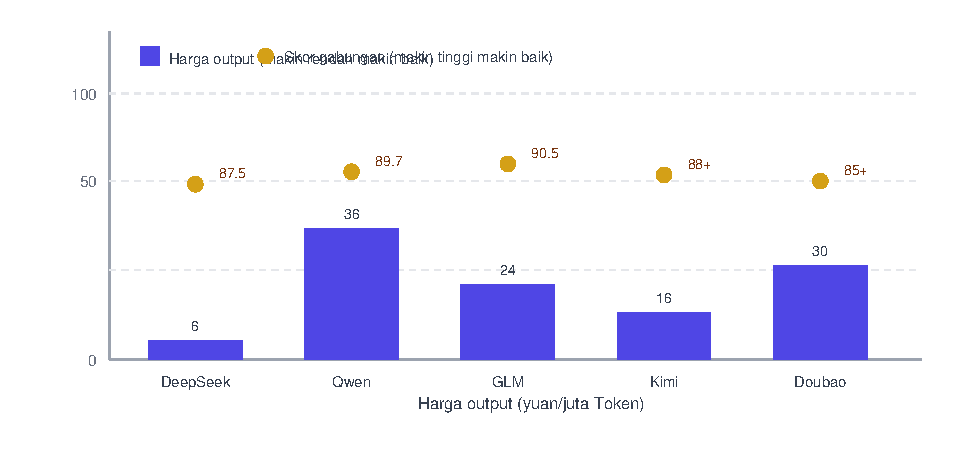
\includegraphics[width=0.92\linewidth]{figures/fig-di-si-shi-er-zhang-1}
\\[2pt]\small Gambar 4: Perbandingan harga dan performa lima model (semakin murah harga semakin baik, semakin tinggi skor semakin baik)
\end{center}

\booksection{Kerangka Keputusan Memilih Model}

Setelah mengenal karakteristik tiap model, bagaimana memilih model untuk proyekmu? Berikan padamu satu “metode keputusan empat pertanyaan” — jawab empat pertanyaan, dan model yang paling cocok untukmu langsung terkunci.

Proyek Anda dipasang di dalam negeri (Tiongkok) atau internasional?

Lokal pilih model dalam negeri

|

Internasional boleh pilih model luar

Tugas utamanya coding atau lainnya?

Coding Claude atau DeepSeek

|

Lainnya lanjut menilai

Butuh konteks super panjang (>500K Token)?

Perlu Gemini atau Kimi

|

Tidak perlu lanjut menilai

Anggaran ketat?

Sensitif DeepSeek atau Qwen-turbo

|

Tidak sensitif GPT-5.6 atau Claude

\begin{center}\small\color{gray}Gambar 5: Metode Keputusan Empat Pertanyaan untuk Memilih Model Besar\end{center}

\begin{tcbinfo}{Tips: Strategi Kombinasi}
Metode ini bukan ajaran mati — banyak skenario justru membutuhkan kombinasi beberapa model. Satu strategi kombinasi yang umum: pakai DeepSeek atau Qwen untuk pengembangan harian (biaya murah, bahasa Tionghoa bagus), Claude untuk desain arsitektur krusial (reasoning kuat, halusinasi rendah), dan Gemini untuk analisis multimodal (pemrosesan gambar dan video). Ganti model sesuai kebutuhan, jangan “satu model dipakai sampai mati”.

\end{tcbinfo}

\booksection{Dasar-Dasar Panggilan API: Menghubungkan Model Besar dari Nol}

Banyak tutorial pemrograman AI hanya mengajarkan cara memakai antarmuka obrolan, tetapi “pemrograman AI” yang sesungguhnya — membuat aplikasimu memanggil model besar — membutuhkan API. API (Application Programming Interface, antarmuka pemrograman aplikasi) adalah protokol komunikasi antar program. Melalui API, kode kamu bisa memanggil kemampuan model besar seperti memanggil sebuah fungsi.

\booksubsection{Apa Itu Token}

Sebelum mengenal API, kamu wajib memahami dulu konsep “Token”. Token adalah satuan dasar penagihan model besar; bisa dipahami sebagai “satuan baca dan tulis AI”. Satu Token kira-kira setara dengan 0,75 kata bahasa Inggris (4 karakter), atau 0,5-1 aksara Tionghoa. Satu teks Tionghoa sepanjang 1000 karakter mengonsumsi sekitar 1500-2000 Token.

Token bukan jumlah kata dan bukan pula jumlah karakter. Model besar memakai tokenizer khusus untuk memotong teks menjadi Token. Kata yang sama bisa memiliki jumlah Token berbeda di tiap model — misalnya “kecerdasan buatan” dalam bahasa Tionghoa mungkin 3 Token di GPT tetapi 2 Token di DeepSeek. API kebanyakan model mengembalikan jumlah Token yang benar-benar terpakai, dan kamu bisa melihatnya di respons API.

\begin{tcbinfo}{Perkiraan Cepat Biaya Token}
1 juta karakter teks Tionghoa kira-kira setara 1,5 juta Token. Memproses input 1 juta karakter + output 1 juta karakter dengan DeepSeek V4 Flash berbiaya sekitar 0,42 dolar AS (sekitar 3 yuan); dengan Claude Fable 5 untuk jumlah yang sama berbiaya sekitar 60 dolar AS (sekitar 434 yuan). Inilah alasan pemilihan model berdampak langsung pada biaya proyekmu.

\end{tcbinfo}

\booksubsection{Mendapatkan API Key}

Langkah pertama memakai API model besar adalah mendapatkan API Key — serangkaian kunci untuk autentikasi identitas. Setiap penyedia model punya platform API sendiri; kamu perlu mendaftar akun dan membuat API Key. Berikut pintu masuk platform API model-model utama beserta proses mendapatkannya:

\begin{center}
\begin{tabularx}{\linewidth}{|X|X|X|X|}
\hline
\textbf{Model} & \textbf{Platform API} & \textbf{Proses Mendapatkan} & \textbf{Kuota Gratis} \tabularnewline
\hline
DeepSeek & platform.deepseek.com & Daftar Verifikasi identitas Buat API Key & Kuota bonus pengguna baru \tabularnewline
Tongyi Qianwen & bailian.aliyun.com (platform Bailian) & Login akun Alibaba Cloud Aktifkan layanan Buat Key & Uji coba gratis pengguna baru \tabularnewline
Zhipu GLM & open.bigmodel.cn & Daftar Verifikasi identitas Buat API Key & Kuota bonus pengguna baru \tabularnewline
Kimi & platform.moonshot.cn & Daftar Verifikasi identitas Buat API Key & Kuota gratis terbatas \tabularnewline
Doubao & volcengine.com (Volcengine) & Daftar Aktifkan layanan Ark Buat API Key & Bonus Token berlimpah saat mendaftar \tabularnewline
OpenAI GPT & platform.openai.com & Daftar Hubungkan kartu kredit Buat API Key & Tanpa kuota gratis (berbayar) \tabularnewline
Anthropic Claude & console.anthropic.com & Daftar Hubungkan kartu Buat API Key & Kuota kecil untuk pengguna baru \tabularnewline
\hline
\end{tabularx}
\end{center}

\begin{center}\small\color{gray}Platform API model utama dan cara mendapatkan Key (Agustus 2026)\end{center}

\textbf{Peringatan Keamanan: API Key = Kata Sandi Dompetmu}\par

API Key setara dengan kata sandi dompetmu — siapa pun yang mendapatkan Key bisa memakai kuotamu untuk memanggil model. Karena itu: jangan pernah menuliskan API Key di dalam kode (kelola dengan environment variable); jangan pernah meng-commit kode yang berisi Key ke repositori Git publik; jangan pernah membagikan tangkapan layar yang memuat Key di media sosial. Jika Key bocor, segera hapus di platform dan buat yang baru.

\booksubsection{Panggilan API Pertama}

Setelah mendapatkan API Key, kamu bisa memanggil API model besar dengan bahasa pemrograman apa pun. Berikut contoh pemanggilan paling sederhana dengan Python — mengirim satu pesan ke DeepSeek dan menerima balasannya.

\begin{lstlisting}[language=Python]
# Pasang SDK: pip install openai
# DeepSeek kompatibel dengan format OpenAI SDK, bisa langsung dipakai
from openai import OpenAI
import os

# 1. Buat client (API Key dibaca dari environment variable)
client = OpenAI(
    api_key=os.environ.get("DEEPSEEK_API_KEY"),
    base_url="https://api.deepseek.com"
)

# 2. Kirim permintaan
response = client.chat.completions.create(
    model="deepseek-chat",  # pilih model
    messages=[
        {"role": "system", "content": "Kamu asisten coding Python."},
        {"role": "user", "content": "Buatkan fungsi quick sort."}
    ]
)

# 3. Ambil balasan
print(response.choices[0].message.content)

# 4. Lihat pemakaian Token
print(f"Token masuk: {response.usage.prompt_tokens}")
print(f"Token keluar: {response.usage.completion_tokens}")
print(f"Total Token: {response.usage.total_tokens}")
\end{lstlisting}

Logika inti kode ini: buat client (membawa API Key dan alamat model) susun daftar pesan (system menentukan peran, user adalah input pengguna) kirim permintaan terima balasan. Pola ini berlaku hampir untuk semua model yang kompatibel dengan format OpenAI — cukup ganti api\_key dan base\_url untuk beralih model. Inilah alasan banyak model buatan Tiongkok memilih kompatibel dengan format OpenAI SDK: pengembang cukup mengubah dua baris kode untuk berganti model, biaya migrasinya sangat rendah.

Berikut perbedaan kode saat beralih ke model lain — perhatikan, hanya dua baris yang perlu diubah:

\begin{lstlisting}[language=Python]
# DeepSeek
client = OpenAI(
    api_key=os.environ.get("DEEPSEEK_API_KEY"),
    base_url="https://api.deepseek.com"
)
# model="deepseek-chat"

# Qwen (platform Bailian)
client = OpenAI(
    api_key=os.environ.get("DASHSCOPE_API_KEY"),
    base_url="https://dashscope.aliyuncs.com/compatible-mode/v1"
)
# model="qwen-plus"

# Zhipu GLM
client = OpenAI(
    api_key=os.environ.get("GLM_API_KEY"),
    base_url="https://open.bigmodel.cn/api/paas/v4"
)
# model="glm-4"

# OpenAI GPT
client = OpenAI(
    api_key=os.environ.get("OPENAI_API_KEY"),
    # base_url cukup pakai nilai default
)
# model="gpt-5.6-terra"
\end{lstlisting}

\booksubsection{Menangani Respons Streaming}

Dalam aplikasi nyata, kamu biasanya tidak ingin menunggu AI menyelesaikan seluruh isinya sebelum ditampilkan sekaligus — itu membuat pengguna menunggu terlalu lama. Respons streaming (Streaming) memungkinkanmu menampilkan teks kata demi kata bersamaan dengan proses pembuatan oleh AI, meningkatkan pengalaman pengguna secara drastis. Seperti mesin tik, huruf-huruf muncul satu per satu, dan rasanya benar-benar berbeda bagi pengguna.

\begin{lstlisting}[language=Python]
# Respons streaming: keluar per karakter
stream = client.chat.completions.create(
    model="deepseek-chat",
    messages=[
        {"role": "user", "content": "Buatkan tutorial bubble sort dengan Python"}
    ],
    stream=True  # aktifkan streaming
)

# terima per blok lalu cetak
for chunk in stream:
    if chunk.choices[0].delta.content is not None:
        print(chunk.choices[0].delta.content, end="", flush=True)
# hasilnya muncul per karakter seperti mesin tik
\end{lstlisting}

\booksection{Panduan Membeli Token Plan}

Sebagian besar penyedia model punya dua cara penagihan: bayar sesuai pemakaian (Pay-as-you-go) dan langganan paket (Token Plan / Subscription). Memahami perbedaan keduanya bisa membantumu menekan biaya penggunaan secara signifikan.

\booksubsection{Bayar per Pemakaian vs Langganan Paket}

\begin{center}
\begin{tabularx}{\linewidth}{|X|X|X|}
\hline
\textbf{Aspek} & \textbf{Bayar per pemakaian (Pay-as-you-go)} & \textbf{Langganan paket (Subscription)} \tabularnewline
\hline
Cara Penagihan & Bayar sesuai jumlah Token yang dipakai & Bayar di muka dengan biaya tetap, dapatkan kuota \tabularnewline
Skenario yang Cocok & Pemakaian tidak stabil, pemanggilan sesekali & Pemakaian stabil, pemanggilan frekuensi tinggi \tabularnewline
Keunggulan Harga & Harga standar & 20\%-50\% lebih murah daripada bayar per pemakaian \tabularnewline
Fleksibilitas & Bisa dipakai kapan saja, tanpa komitmen & Perlu bayar di muka; kuota yang kedaluwarsa bisa hangus \tabularnewline
Penanganan Kelebihan Kuota & Otomatis ditagih per pemakaian & Setelah kuota habis, beralih ke bayar per pemakaian \tabularnewline
Contoh Platform & Platform API resmi masing-masing model & OpenAI Plus/Pro, Claude Pro, Cursor Pro \tabularnewline
\hline
\end{tabularx}
\end{center}

\begin{center}\small\color{gray}Perbandingan dua cara penagihan\end{center}

Untuk pemula, sebaiknya mulai dari bayar per pemakaian — tanpa perlu bayar di muka, pakai seberapa banyak bayar seberapa banyak. Setelah volume pemakaian bulananmu stabil di satu level (misalnya di atas 50 yuan per bulan), barulah pertimbangkan beralih ke langganan paket untuk mendapatkan harga satuan yang lebih murah.

\booksubsection{Ikhtisar Paket Langganan Utama}

\begin{center}
\begin{tabularx}{\linewidth}{|X|X|X|X|}
\hline
\textbf{Paket} & \textbf{Biaya Bulanan} & \textbf{Yang Termasuk} & \textbf{Cocok Untuk} \tabularnewline
\hline
ChatGPT Free & Gratis & Obrolan teks tanpa batas dengan GPT-5.6 Luna & Mencoba dari nol \tabularnewline
ChatGPT Plus & US\$20/bulan & GPT-5.6 Sol, pembuatan gambar, analisis data, akses plugin & Pengguna menengah \tabularnewline
ChatGPT Pro & US\$200/bulan & Pakai semua model tanpa batas, akses prioritas ke fitur baru & Pengguna profesional berat \tabularnewline
Claude Free & Gratis & Obrolan Claude dengan jumlah terbatas & Mencoba dari nol \tabularnewline
Claude Pro & US\$20/bulan & Pakai Claude tanpa batas, akses prioritas ke model baru & Pengembang yang coding \tabularnewline
Cursor Free & Gratis & Pelengkapan dan obrolan AI dengan jumlah terbatas & Coba-coba pemula \tabularnewline
Cursor Pro & US\$20/bulan & Pelengkapan AI tanpa batas, 500 permintaan premium per bulan & Pengembang sehari-hari \tabularnewline
Cursor Business & US\$40/bulan/orang & Kolaborasi tim, panel admin, mode privasi & Penggunaan tim \tabularnewline
\hline
\end{tabularx}
\end{center}

\begin{center}\small\color{gray}Paket langganan alat AI utama (Agustus 2026)\end{center}

Skema langganan model dalam negeri (Tiongkok) sedikit berbeda. DeepSeek terutama memakai bayar per pemakaian tanpa paket langganan bulanan — kamu mengisi saldo dan biaya dipotong sesuai pemakaian nyata. Tongyi Qianwen menyediakan paket sumber daya prabayar di platform Bailian (membeli kuota Token tertentu dengan harga diskon). Doubao di Volcengine juga punya skema prabayar serupa. Bagi pengembang di Tiongkok, kombinasi paling hemat biasanya: DeepSeek bayar per pemakaian (pengembangan harian) + kuota gratis Doubao (uji coba).

\booksubsection{Platform Agregator API}

Jika kamu perlu memakai beberapa model sekaligus, platform agregator API adalah pilihan yang praktis. Platform agregator memberikan satu API Key terpadu sehingga kamu bisa memanggil puluhan model dari seluruh dunia tanpa harus mendaftar di tiap platform.

\begin{center}
\begin{tabularx}{\linewidth}{|X|X|X|X|}
\hline
\textbf{Platform} & \textbf{Keunggulan} & \textbf{Keunggulan Harga} & \textbf{Skenario yang Cocok} \tabularnewline
\hline
OpenRouter (openrouter.ai) & Platform agregator internasional; satu Key untuk memanggil model dari seluruh dunia & Harga transparan, bisa membandingkan harga real-time & Perlu beralih secara fleksibel antar banyak model luar negeri \tabularnewline
SiliconFlow (siliconflow.cn) & Platform agregator Tiongkok, menyediakan API berbagai model buatan Tiongkok & 20\%-30\% lebih murah daripada harga resmi & Pengembang di Tiongkok yang ingin membandingkan harga antar model \tabularnewline
Azure OpenAI (proxy Microsoft) & API OpenAI via proxy Microsoft Azure & Batch API bisa setengah harga & Panggilan OpenAI tingkat enterprise, tugas asinkron bervolume besar \tabularnewline
Baidu Qianfan (qianfan.baidubce.com) & Platform AI Cloud Baidu, menyediakan model seperti Wenxin (ERNIE) & Kuota gratis untuk pengguna baru & Pengguna ekosistem Baidu \tabularnewline
\hline
\end{tabularx}
\end{center}

\begin{center}\small\color{gray}Platform agregator API populer (Agustus 2026)\end{center}

\textbf{Peringatan jebakan: jangan beli “Key bersama”}\par

Jangan membeli yang namanya “API Key bersama” di platform seperti Taobao atau Xianyu—Key semacam ini biasanya berasal dari sumber yang tidak jelas, bisa kapan saja diblokir, dan berisiko membocorkan data. Selalu dapatkan API Key melalui platform resmi atau platform agregator yang kredibel.

\booksubsection{Strategi optimasi biaya}

Memilih model yang tepat hanyalah langkah pertama; cara “memakainya secara hemat” sama pentingnya. Berikut beberapa strategi optimasi biaya yang sudah teruji di praktik:

\begin{enumerate}
  \item Manfaatkan cache hit. Banyak model menyediakan fitur "cache"—ketika permintaanmu memuat konten yang sudah pernah diproses sebelumnya (seperti system prompt), bagian itu hanya ditagih dengan harga sangat rendah. Harga cache hit DeepSeek hanya 1/60 dari harga normal. Letakkan system prompt yang tetap di awal daftar pesan agar cache hit maksimal.
  \item Routing berjenjang—pakai model murah untuk tugas sederhana dan model mahal untuk tugas kompleks. Misalnya, pakai DeepSeek V4 Flash untuk klasifikasi teks (output 2 yuan/juta token) dan Claude untuk desain arsitektur (output 181 yuan/juta token). Sekitar 80\% panggilan dalam satu proyek bisa memakai model murah.
  \item Batasi panjang output. API ditagih berdasarkan token output; semakin panjang, semakin mahal. Pada skenario yang tidak butuh penjelasan panjang lebar, atur parameter max\_tokens untuk membatasi panjang output agar AI tidak "terlalu banyak basa-basi".
  \item Gunakan Batch API untuk tugas non-real-time. Jika kamu punya banyak tugas yang tidak butuh respons seketika (misalnya pelabelan data massal atau ringkasan dokumen), Batch API memberikan diskon 50\%. OpenAI dan Azure sama-sama menyediakan fitur ini.
  \item Pantau pemakaian token. Sebagian besar platform API menyediakan dasbor statistik pemakaian. Periksa berkala distribusi pemakaiannya, cari panggilan yang paling boros token, lalu optimalkan secara terarah. Satu penyesuaian kecil pada prompt (misalnya mengganti "jelaskan secara rinci" dengan "jelaskan dalam 3 kalimat") bisa menghemat 50\% token.
\end{enumerate}

\begin{center}
\begin{tabularx}{\linewidth}{|X|X|X|X|}
\hline
\textbf{Strategi optimasi} & \textbf{Penghematan} & \textbf{Tingkat kesulitan} & \textbf{Keterangan} \tabularnewline
\hline
Cache hit & Hingga 98\% & Rendah & Letakkan konten yang tetap di awal pesan \tabularnewline
Routing berjenjang & 50\%-80\% & Sedang & Model murah untuk tugas sederhana \tabularnewline
Batasi panjang output & 30\%-60\% & Rendah & Atur parameter max\_tokens \tabularnewline
Batch API & 50\% & Rendah & Batch untuk tugas non-real-time \tabularnewline
Optimasi prompt & 20\%-50\% & Sedang & Padatkan prompt, kurangi bagian berlebih \tabularnewline
\hline
\end{tabularx}
\end{center}

\begin{center}\small\color{gray}Strategi optimasi biaya dan hasilnya (Agustus 2026)\end{center}

\booksection{Praktik: menghubungkan API model besar ke proyek}

Mari akhiri bab ini dengan satu praktik lengkap—membuat “Generator Ringkasan AI”: pengguna memasukkan sepotong teks panjang, lalu program memanggil API model besar untuk menghasilkan ringkasan. Praktik ini memperlihatkan alur lengkap pemanggilan API: konfigurasi lingkungan, pemanggilan API, penanganan error, dan kontrol biaya.

\begin{lstlisting}[language=Python]
# ai_summarizer.py - peringkas teks AI
import os
from openai import OpenAI

# 1. Konfigurasi (baca API Key dari environment variable, jangan pernah hardcode)
client = OpenAI(
    api_key=os.environ.get("DEEPSEEK_API_KEY"),
    base_url="https://api.deepseek.com"
)

def summarize(text: str, max_length: int = 200) -> dict:
    """Meringkas teks

    Args:
        text: teks asli yang akan diringkas
        max_length: panjang ringkasan maksimum (jumlah Token)

    Returns:
        dict: berisi ringkasan dan info pemakaian Token
    """
    try:
        response = client.chat.completions.create(
            model="deepseek-chat",
            messages=[
                {
                    "role": "system",
                    "content": "Kamu adalah generator ringkasan."
                               "Rangkum teks yang diberikan pengguna secara ringkas."
                               "Ringkasan tidak lebih dari 3 kalimat."
                },
                {
                    "role": "user",
                    "content": f"Ringkas teks berikut:\n\n{text}"
                }
            ],
            max_tokens=max_length,  # batasi panjang keluaran
            temperature=0.3  # suhu rendah=lebih stabil
        )

        return {
            "success": True,
            "summary": response.choices[0].message.content,
            "input_tokens": response.usage.prompt_tokens,
            "output_tokens": response.usage.completion_tokens,
            "total_tokens": response.usage.total_tokens
        }

    except Exception as e:
        return {
            "success": False,
            "error": str(e)
        }

# 2. Contoh pemakaian
if __name__ == "__main__":
    long_text = """
    (tempel teks panjang di sini...)
    """

    result = summarize(long_text)

    if result["success"]:
        print(f"Ringkasan: {result['summary']}")
        print(f"Token terpakai: {result['total_tokens']}")
        # estimasi biaya: DeepSeek V4 Flash
        cost = result['total_tokens'] * 0.000004  # sekitar 0.4 sen per seribu Token
        print(f"Estimasi biaya: {cost:.4f} yuan")
    else:
        print(f"Terjadi kesalahan: {result['error']}")
\end{lstlisting}

Kode ini mencerminkan beberapa praktik terbaik pemanggilan API: API Key dibaca lewat environment variable, tidak pernah ditulis langsung di dalam kode; fungsi dilengkapi dokumentasi dan type hint yang jelas; max\_tokens diatur untuk membatasi panjang output; temperature diatur rendah (0.3) agar output lebih stabil; penanganan error lengkap; dan informasi konsumsi token dikembalikan untuk pelacakan biaya. Saat kamu memakai AI untuk menulis kode ini, sampaikan saja persyaratan-persyaratan tersebut—AI sepenuhnya mampu mewujudkannya untukmu.

Pelajaran terakhir bab ini: model adalah "amunisi", metodologi adalah "taktik". Memilih amunisi yang tepat membuat pertempuran lebih lancar, tetapi tanpa taktik yang baik, amunisi sebanyak apa pun tak akan menang. Setelah mengenal karakter tiap model dan cara memakai API, Anda punya "gudang amunisi" yang cukup—tetapi bagaimana memenangkan pertempurannya tetap bergantung pada metodologi berpikir yang dipelajari di bab-bab sebelumnya.

\begin{tcbpractice}{Mari praktik: buat panggilan API pertamamu berhasil}
Daftar di satu platform model dalam negeri (disarankan DeepSeek atau Zhipu—keduanya memberi kuota gratis bagi pengguna baru), buat API Key, tuliskan ke environment variable sistem (bukan ke dalam kode!), lalu jalankan kode “panggilan API pertama” di atas. Pada saat jawaban AI berhasil tercetak, kamu sudah melewati garis batas antara “memakai AI” dan “membangun aplikasi AI”.

\end{tcbpractice}

\begin{tcbsummary}{Ringkasan bab ini}
\begin{itemize}
  \item Tiga raksasa internasional: GPT-5.6 (seimbang dan serba bisa), Claude (puncak kemampuan coding + tingkat halusinasi hanya 1\%), Gemini (raja multimodal + konteks 2 juta)
  \item Lima raksasa dalam negeri: DeepSeek V4 (raja value for money, perhatikan pengumuman kenaikan harga), Qwen3.7 (kelas enterprise), GLM-5.1 (nomor satu dalam negeri untuk SWE), Kimi K3 (teks super panjang), Doubao (gratis untuk pemula)
  \item Metode keputusan empat pertanyaan: di-deploy di mana? untuk coding atau lainnya? butuh konteks super panjang? sensitif terhadap anggaran?
  \item Token adalah satuan penagihan: 1 karakter Mandarin sekitar 1,5-2 token; 1 juta karakter sekitar 1,5 juta token
  \item API Key = sandi dompetmu: kelola lewat environment variable, jangan pernah ditulis langsung di kode, jangan diunggah ke Git
  \item Model dalam negeri umumnya kompatibel dengan OpenAI SDK: mengganti model cukup dengan mengubah dua baris, api\_key dan base\_url
  \item Lima cara hemat: cache hit, routing berjenjang, batasi output, Batch API, pantau pemakaian
\end{itemize}

\end{tcbsummary}
